\section{Finding moving objects in an image (field of view)}
\setcounter{questions}{1}


  This exercise introduces the Sky Body Tracker (\skybot) tool
  \citep{2006-ASPC-351-Berthier}.
  \skybot is a specialized \texttt{cone-search}: it lists
  all Solar System Objects (SSOs) present within
  a given field of view \textbf{at a given epoch}.
  Alike all the services hosted at
  \href{https://www.imcce.fr}{IMCCE}
  on the VO Solar System Portal
  %(\href{https://ssp.imcce.fr/webservices/}{VOSSP}),
  (VOSSP\footnote{Forms: \href{https://ssp.imcce.fr/forms}{https://ssp.imcce.fr/forms}\\
  \hspace*{1.8em}APIs: \href{https://ssp.imcce.fr/webservices}{https://ssp.imcce.fr/webservices}}),
  \skybot requests
  can be submitted in different ways
  (\aladin, HTTP, SOAP), and results can be provided in different 
  formats (\href{https://www.ivoa.net/documents/VOTable/}{VOTable}, text, html).\\

  We will use \skybot to illustrate calls to VO services first with
  a graphical user interface (GUI), \aladin (Fig.~\ref{fig:aladin}), then 
  with a \python script (in the \BC{XXX} notebook).


%%%--------------------------------------------------------------------------------
\begin{figure}[ht]
  \centering
  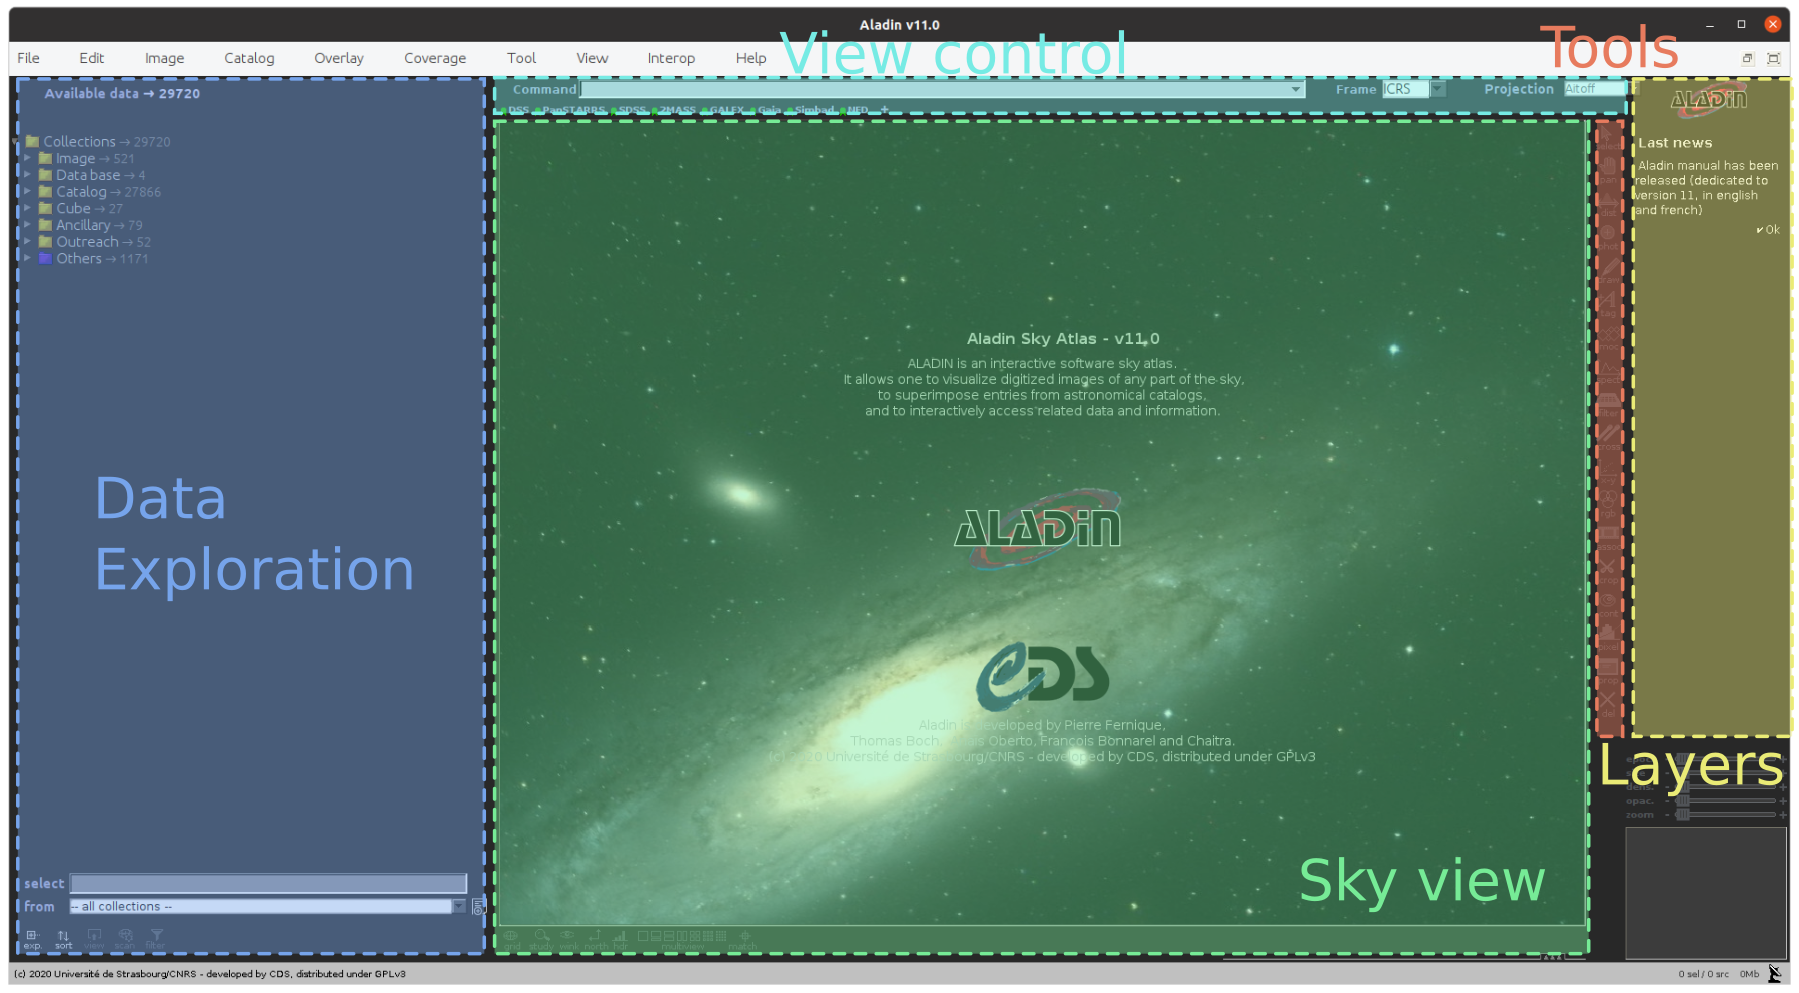
\includegraphics[width=0.8\hsize]{aladin}
  \caption{The \aladin client. Loaded data from the
  \texttt{data exploration} panel are listed as
  \texttt{layers} and displayed in the  
  \texttt{sky view}. Coordinates can be entered in the
  \texttt{view control} panel, and many
  \texttt{tools} are available.
  }
  \label{fig:aladin}
\end{figure}
%%%--------------------------------------------------------------------------------

\newpage
  \begin{enumerate}
    \setlength\itemsep{0em}
    \item Launch \aladin.

    \item Using the \texttt{view control}, center de view on (RA,Dec) of (07h 08m, +26d 34m).

    \item Open the \texttt{Serveur selector}. Keystroke \texttt{ctrl-l} or \texttt{File} 
      $\rightarrow$ \texttt{Open server selector}.
  \end{enumerate}
  \setcounter{saveitem}{\value{enumi}}  

%%%--------------------------------------------------------------------------------
\begin{wrapfigure}[11]{r}{0.4\textwidth}
  \vspace{-2.5em}
  \begin{center}
    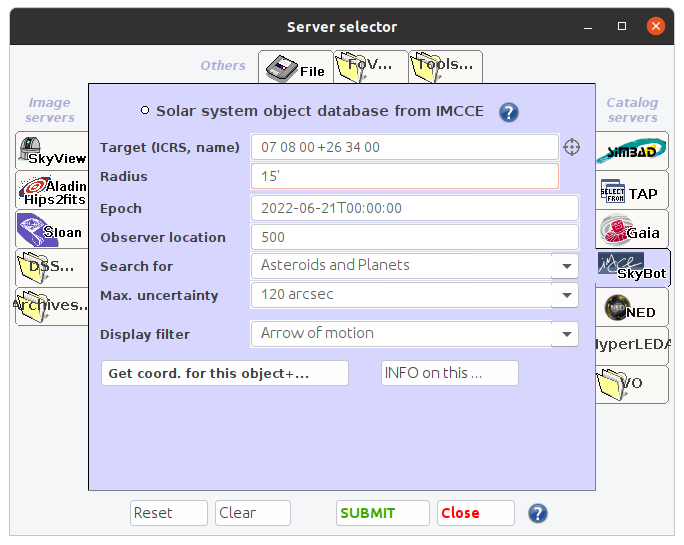
\includegraphics[width=\hsize]{skybot-server_selector}
  \end{center}
\end{wrapfigure}
%%%--------------------------------------------------------------------------------

  There are seven fieds in the pop-up window:
  \texttt{Target},
  \texttt{Radius},
  \texttt{Epoch},
  \texttt{Observer location},
  \texttt{Search For},
  \texttt{Max. uncertainty}, and
  \texttt{Display filter}.
  By default, \aladin fills the
  \texttt{Target} and
  \texttt{Radius} fields to correspond to current display.

  \begin{enumerate}
    \setlength\itemsep{0em}
    \setcounter{enumi}{\value{saveitem}}
    \item Check that the coordinates in \texttt{Target} correspond to the value above.

    \item Set the \texttt{Radius} to \texttt{15'}.

    \item Set the \texttt{Epoch} to \texttt{2022-06-21T00:00:00}.

    \item Let everything else by default and click on \texttt{SUBMIT}.
  \end{enumerate}
  \setcounter{saveitem}{\value{enumi}}  

  A new layer has appeared, showing the SSOs with their
  arrow of motion. Like for any other catalog loaded in \aladin,
  you can select objects and see their properties in the bottom panel.

  \begin{enumerate}
    \setlength\itemsep{0em}
    \setcounter{enumi}{\value{saveitem}}
    \item Select all SSOs. \texttt{Ctrl-a} or \texttt{Edit} $\rightarrow$ \texttt{Select all objects}.

    \item Click on any of the column in the bottom panel. The histogram of values for all 
      objects will appear at the bottom right.
  \end{enumerate}
  \setcounter{saveitem}{\value{enumi}}  


  \BC{give a sentence on aladin as general? Outside the scope of the present tutorial, but many
  options on projection, background image, field of view, catalogs? 
  Give the link to a tutorial specifically on aladin?}




\section{In a script}

We often process many images. Clicking on a GUI is not the most
productive method. We thus often write scripts to perform
many automated steps. Most VO services can be called through APIs
and be scripted.

Generally, the service has a base \texttt{url} to which queries are
to be sent. The user choices are submitted through a list of \texttt{parameter}=\texttt{value}
arguments. Of course, we cannot guess which \texttt{parameter} is
available, nor what \texttt{value} are allowed. So read the documentation!

For instance, we can repeat the query above in \python:

\begin{lstlisting}[language=python]
import requests
import json
import pandas as pd
from astropy.coordinates import Angle

# User choices
ep = '2022-06-21T00:00:00'
ra = '07h08m00'
dec = '+26d34m00'
sr = 15/60
observer = '500'

# Service URL
url = 'http://vo.imcce.fr/webservices/skybot/skybotconesearch_query.php?'

# Query parameters
params = {
     '-ep': ep,
     '-ra': Angle(ra).degree,
     '-dec': Angle(dec).degree,
     '-sr': sr,
     '-mime': 'text',
     '-output': 'all',
     '-loc': observer, 
     '-tscale': 'UTC'
    }

# Query the service
r = requests.post(url, params=params, timeout=2000)

# Write results to disc
with open("response.txt", "w") as f:
    f.write(r.text)

# Load results in a pandas.DataFrame
data = pd.read_csv( 'response.txt', sep='|', skiprows=2 )
\end{lstlisting}

  So long story short, we first
  define the parameters (coordinates, radius, epoch) then query the
  \skybot service thanks to the \texttt{request} package. The results
  are written in a file, and read as a \texttt{pandas} \texttt{DataFrame}.
  Performing this query for each image acquired by a telescope is very easy
  (the parameters are contained in the image).
